\chapter{\label{ch:1-intro}Introduction} 
\minitoc
\section{Astrophysics in the Gamma-Ray Domain}
A wide variety of astrophysical objects produce gamma-rays, including supernova remnants, activate galactic nuclei (AGN) and pulsars (to name but a few) \cite{scienceCTA}. In order to fully understand these objects, we need to capture maximal information about their emission, across the electromagnetic spectrum, as well as with multi-messenger methods (neutrinos, gravitational waves and cosmic rays).  However, performing electromagnetic observations of these sources at very high photon energies is difficult for a number of reasons \cite{jamieiact}. Firstly, these gamma rays can't be focused and as such it is necessary to use particle physics techniques to reconstruct their point of origin. Secondly, gamma rays do not penetrate the Earth's atmosphere, meaning that in order to detect gamma rays directly the instrument must be in space. Finally, gamma rays are comparatively rare (the brightest astrophysical gamma-ray sources have a flux of about 6 $\rm{photons} \ \rm{m}^{-2}\ \rm{year}^{-1}$ above 1TeV\cite{jamieiact}), meaning that in order to detect the highest energy gamma-rays one must use an instrument with a very large effective area.

\subsection{The Fermi Space Telescope}
The first two of these problems can be solved by observing in space, and the very successful Fermi mission has operated for over a decade. However, the energy range of its Large Area Telescope (LAT) survey instrument is limited to between 20MeV and 300GeV because of the comparatively small effective of the detector. As such, in order to observe higher energy photons (in the high GeV-TeV energy range) we must detect them indirectly. This can be performed using the Imaging Atmospheric Cherenkov Telescope  (IACT) method, pioneered by Jelly and Galbraith in 1953 \cite{G+J}. 

\section{Current Generation Indirect Gamma-ray Detection Instruments}
\subsection{The Cherenkov Effect}

\begin{figure}[ht] 
        % read manual to see what [ht] means and for other possible options
        \centering 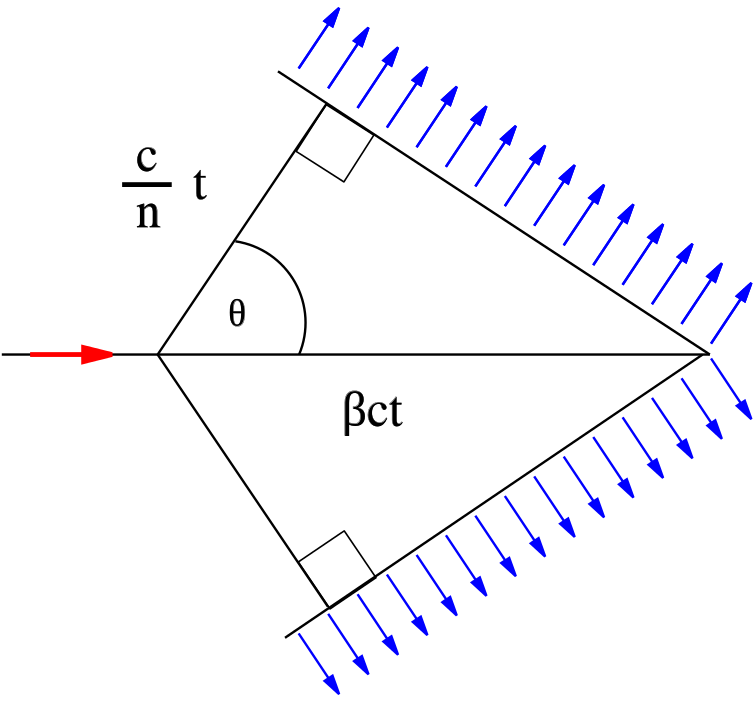
\includegraphics[width=0.5\columnwidth]{figures/Cherenkov.png}

        % note that in above figure file name, "sr_setup",
        % the file extension is missing. LaTeX is smart enough to find
        % apropriate one (i.e. pdf, png, etc.)
        % You can add this extention yourself as it seen below
        % both notations are correct but above has more flexibility
        %\includegraphics[width=1.0\columnwidth]{sr_setup.pdf}
        \caption{
                \label{fig:cherenkov} % spaces are big no-no withing labels
                % things like fig: are optional in the label but it helps
                % to orient yourself when you have multiple figures,
                % equations and tables
                The geometry of the Cherenkov effect, assuming no dispersion. Image credit: A. Horvarth.
        }
\end{figure}
The Cherenkov opening angle $\theta_c$
\begin{equation}
    \cos\theta_c=\frac{1}{n\beta}
    \label{eq:cherenkov}
\end{equation}

where $n$ is the refractive index, $\beta$=$v/c$ where $v$ is the velocity of light in the medium and $c$ is the speed of light in a vacuum.
\hl{Complete this section}
The energy $dE$ emitted as a result of the particle traversing the medium per unit length $dx$ is given by the Frank-Tamm formula, derived in 1937 (and winning the authors a Nobel prize in 1958), which holds provided the velocity $v$ as a fraction of the speed of light in a vacuum $c$ is greater than $\frac{1}{n(\omega})$ (where $n(\omega)$ is the frequency dependent refractive index)
\begin{equation}
    \frac{d^2E}{dx\ d\omega}=\frac{q^2}{4\pi}\mu(\omega)\omega\left(1- \frac{c^2}{v^2(\omega)} \right)
    \label{eq:FT}
\end{equation}
where $\mu(\omega)$ is the frequency dependent permeability, and $q$ is the charge of the particle \cite{franktamm}. The total energy emitted in Cherenkov radiation is therefore given by the corresponding integral
\begin{equation}
    \frac{dE}{dx}=\frac{q^2}{4\pi}\int_{v>\frac{c}{n(\omega)}}^{\infty}\mu(\omega)\omega \left(1- \frac{c^2}{v^2n^2(\omega)} \right) d \omega .
    \label{eq:FT2}
\end{equation}

This integral is finite as $\lim_{\omega \to \infty} n(\omega)<1$ and $\lim_{\omega \to 0} n(\omega)=1$ . Assuming $\mu(v)$ is unity equation \ref{eq:FT} can also be integrated over frequency \cite{katz} to get the number of Cherenkov photons $dN_{\gamma}$ emitted per unit length
\begin{equation}
    \frac{dN_{\gamma}}{dx}=2\pi\alpha \left( 1- \frac{1}{\beta^2n^2} \right) \left(\frac{1}{\lambda_{min}}-\frac{1}{\lambda_{max}} \right)
\end{equation}
where $\alpha$ is the fine structure constant, and the $\lambda$ terms represent the minimum and maximum wavelength range of the emission. Taking this band to be 300nm-600nm and $\beta$=1 implies $\frac{dN_{\gamma}}{dx}$ is around $\mathrm{15 m^{-1}}$ at an 8km altitude in air \cite{katz}. 
\subsection{IACT Basics}

\begin{figure}[ht] 
        % read manual to see what [ht] means and for other possible options
        \centering 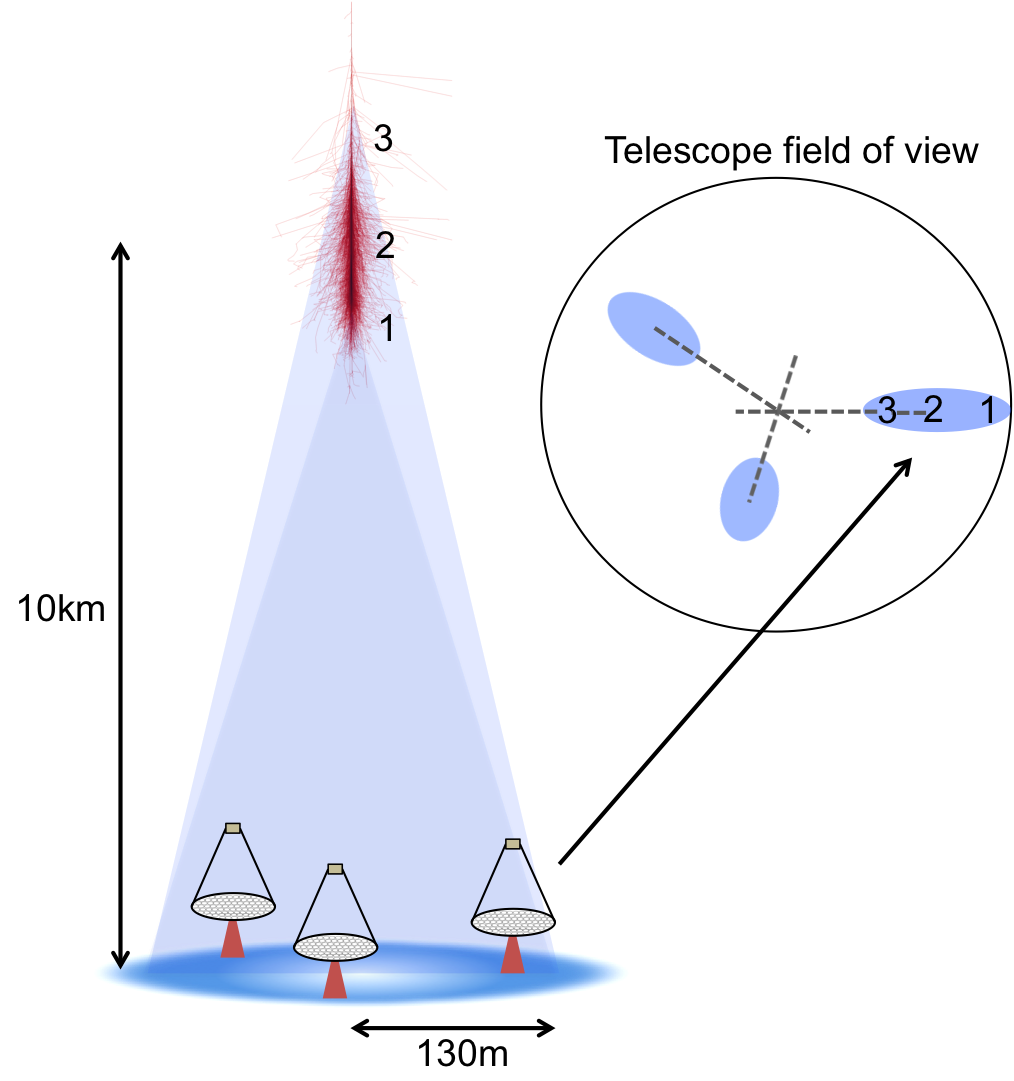
\includegraphics[width=0.7\columnwidth]{figures/schematic.png}

        % note that in above figure file name, "sr_setup",
        % the file extension is missing. LaTeX is smart enough to find
        % apropriate one (i.e. pdf, png, etc.)
        % You can add this extention yourself as it seen below
        % both notations are correct but above has more flexibility
        %\includegraphics[width=1.0\columnwidth]{sr_setup.pdf}
        \caption{
                \label{fig:schem} % spaces are big no-no withing labels
                % things like fig: are optional in the label but it helps
                % to orient yourself when you have multiple figures,
                % equations and tables
                A schematic of the IACT technique, taken from \cite{jamieiact}. Three telescopes stereoscopically observe a
                Cherenkov light pool caused by an EAS. The direction of the incident photon is reconstructed by intersecting the primary axes of 				 the elliptical images in the three cameras. On the right, an illustration that the light from the lowest altitude part of the shower is the first to arrive on the ground.
        }
\end{figure}
When a photon with an energy of above around 50GeV encounters the Earth's atmosphere, it undergoes pair production in the electric field of the nucleus of an atmospheric molecule $X$
\begin{equation}
\mathrm{\gamma}+\mathrm{X} \rightarrow \mathrm{X}+\mathrm{e^+}+ \mathrm{e^-}.
\end{equation}
This occurs on average after the $\gamma$-ray travels through one radiation length's worth of atmosphere, typically at around a 20km altitude \cite{weekesgamma}. The resulting electron and positron have very high kinetic energy, and so travel very close to the speed of light in a vacuum and faster than the speed of light in air. As a result, Cherenkov radiation is emitted by the molecules in the vicinity of the particle.
%add more depth here
The generated particles continue to interact, emitting photons via Brehmsstrahlung radiation, and creating a particle cascade or Extensive Air Shower (EAS). This cascade continues down into the atmosphere until the radiation and ionisation losses become equal, which is also the point at which the maximum number of particles ($N_{Max}$) are present in the shower as a function of atmospheric mass traversed $X_{Max}$(in $\mathrm{g\ cm^{-2}}$). This point is known as the shower maximum. The altitude at which this occurs is referred to as $h_{Max}$, after which point the energy losses dominate and the number of produced particles significantly reduces. For an incident $\gamma$-ray of 10 TeV energy, $X_{Max}\approx 431 \mathrm{\ g\ cm^{-2}}$, $h_{Max}=6.8\ \mathrm{km}$ and $N_{Max}=1.0 \times 10^4$ \cite{weekesgamma}. Some muons from the shower interaction can however survive to reach the ground, at around a rate of 1 muon a $\mathrm{cm^{-2}}$ minute$^{-1}$. The Cherenkov light produced from this EAS forms a pool on the ground of radius $\sim$120 m \cite{weekesgamma}, and this can be observed with an optical frequency telescope on the ground at night provided it is equipped with an extremely fast (ns timescale) camera, as the Cherenkov light flash from an EAS is of the order of a few ns. In order to reconstruct the energy and direction of the incident $\gamma$-ray optimally, data from an array of such telescopes is typically combined stereoscopically, a technique pioneered by the \textit{High-Energy-Gamma-Ray Astronomy} (HEGRA) instrument in the 1990s \cite{HEGRA}. This use of stereoscopy improves backround rejection power as the chances of directly imaging a muon ring originating from a proton shower are higher, and with multiple images the determination of shower width is more accurate.  The optimal spacing for these telescopes is of the same order as the size of the light pool on the ground \cite{weekesgamma}.

Given that the only interactions possible in an electomagnetic air shower are pair production and $\gamma$-ray brehmstrahlung, it is possible to construct a simple model of their evolution (the Heitler model) \cite{heitler}. Given that the radiation length of an electron in the atmosphere is known, $X_0=\mathrm{36.7\ g\ cm^{-2}}$, the typical length over which a new pair production will occur is $N_0=X_0 \ln 2$, therefore after $n$ interactions the atmospheric grammage traversed is $x=nX_0 \ln 2$, and the number of surviving particles is $N=2^n=\exp \left( \frac{x}{X_0}\right)$. Assuming the particle energies are uniformly distributed, the energy per particle $E=E_0/N$ (where $E_0$ is the initial energy of the originally incident particle. Given that the shower maximum occurs when $E=E_c^e=\mathrm{85 MeV}$, the number of particles at shower maximum is given by 
\begin{equation}
    N_{Max}=2^{n_c}=\frac{E_0}{E_c^e}
\end{equation}
where $n_c=\frac{\ln (\frac{E_0}{E_e^c})}{\ln 2}$.
%Need refs for this bit
\section{Current Generation Instruments}
\subsection{VERITAS}
\textit{Very Energetic Radiation Imaging Telescope Array System} (VERITAS) consists of 4 12 meter parabolic, single mirror IACTs at the Fred Lawrence Whipple Observatory in Arizona (the original VERITAS design intended 8 IACTs). Construction of VERITAS began in 2003 and was completed in 2007. It is designed to give optimal sensitivity in 100GeV to 10TeV energy band. Recent work performed by VERITAS includes the discovery of gamma-ray emission from the Blazar TXS 0506+056, coincident with a neutrino detection from IceCube \cite{TXS}, and the detection of TeV gamma-rays from the Blazar PKS 1441+25, indicating the transparency of the universe to photons of such energies \cite{escape}. In chapter \ref{ch:4-VERITASRealData}, we use real data from VERITAS to test deep learning based event classification as a technique intended for use by CTA.

\subsection{MAGIC}
\textit{Major Atmospheric Gamma Imaging Cherenkov Telescopes} (MAGIC) consists of two 17m IACTs on La Palma, designed to detect $\gamma$-rays with energies between 25GeV and 30 TeV. MAGIC's cameras are unusual as they consist of two separate types of conventional photomultiplier, 386 hexagonal pixels in the centre surrounded by 180 larger pixels at the edge. Primarily constructed to hunt for Gamma-Ray Bursts (GRBs) from the ground, a goal it achieved when it detected TeV $\gamma$-rays from GRB 190114C in early 2019 \cite{magicGRB}.
\subsection{H.E.S.S.}
\textit{High Energy Stereoscopic System} (H.E.S.S.) is an IACT array in the Khomas Highlands of Namibia. The only current generation instrument to consist of multiple classes of IACT, 4 with a $\sim$ 12 meter diameter mirror and a fifth with a 28m diameter mirror, giving it an operational energy range of 30GeV to 100TeV. Construction of the four original 12m instruments was completed in 2003, with the larger telescope completed in 2012. Notable recent achievements of H.E.S.S. include resolving the extension of the Crab Nebula \cite{crabextension} and the jet of Centaurus A \cite{cena}.

\subsection{FACT}
The \textit{First G-APD Cherenkov Telescope} (FACT) is an autonomous upgrade of a former HEGRA Cherenkov telescope, notable for being the first instrument to attempt the use of Silicon Photomultipliers in Cherenkov astronomy. Given it is a single IACT and not an array, however, its sensitivity is limited. As such it largely operates as a blazar monitoring instrument, such that other instruments can be notified in the event of a flare. 

FACT arguably has one of the most advanced analysis chains of current IACTs, which is largely based in Python, and this has had a partial influence on CTA's analysis chain. Notably the FACT collaboration used open source, python-based analysis tools developed using modern version control (with git and github) \cite{factspec}. This was not the case for any of the other analysis chains developed for the other current IACTs which remain largely based on root.

\subsection{HAWC, Tibet AS-$\gamma$ and LHASSO}

The IACT technique is not the only means of indirect $\gamma$-ray detection from the ground. At sufficiently high altitude, one can use Water Cherenkov detectors to directly observe the electrons from an incident shower, and then use arrival time information as a background rejection method. This is the key principle underlying the successful \textit{High Altitude Water Cherenkov} (HAWC) observatory in Mexico, as well the principle behind the Chinese Tibet AS-$\gamma$ and \textit{Large High Altitude Air Shower Observatory} (LHASSO) experiments (the currently under construction LHASSO detector will also have small IACTs on site). These complement IACTs with their main advantage of being that these are survey instruments with a wide field of view, higher operational energy range and nearly $100\%$ duty cycle, but comparatively poor angular resolution and background rejection. 

\section{The Cherenkov Telescope Array and Associated Instruments}
The Cherenkov Telescope Array (CTA) is an ambitious project to build a next-generation VHE $\gamma$-ray facility, which aims to improve on the sensitivity of the current generation instruments by roughly an order of magnitude \cite{scienceCTA}. The CTA consortium, involved in directing CTA Observatory science goals and array design, consists of over 1400 scientists from 31 countries around the globe. Given the large energy range (20 GeV to 300 TeV) that CTA will operate  over \cite{scienceCTA}, three classes of IACT are required. These are designated as the Small-, Medium- and Large-Sized Telescopes (SSTs, MSTs and LSTs). The 23-meter diameter LSTs are designed for high sensitivity observations of $\gamma$-rays over the 20 GeV-150 GeV energy range, increasing the overlap in sensitivity with space based missions such as the Fermi $\gamma$-ray Space Telescope \cite{Fermi}. The SSTs will be the smallest (approximately 4 m diameter) but most numerous telescopes, and will be spread out over a large ($\sim$4 km$^2$) area in order to maximise CTA's effective area for $\gamma$-ray energies over 5 TeV. The MSTs will provide unprecedented sensitivity to cosmic $\gamma$-ray fluxes in the intermediate energy range. The baseline (omega configuration) design of CTA consists of 99 telescopes (4 LSTs, 25 MSTs, 70 SSTs) placed on a southern site at Cerro Paranal in Chile, whereas a smaller array of 19 telescopes (4 LSTs, 15 MSTs, and no SSTs) will be placed on a northern site on Spanish Canary Island of La Palma. By having both a northern and southern site, the CTA Observatory will cover the whole sky \cite{scienceCTA}. However, as of writing this thesis, the current construction plan for CTA is to first build a so called alpha configuration array consisting of 4 LSTs and 9 MSTs in the northern site, and 14 MSTs and 37 SSTs in the southern array.
\begin{figure}[ht] 
        % read manual to see what [ht] means and for other possible options
        \centering 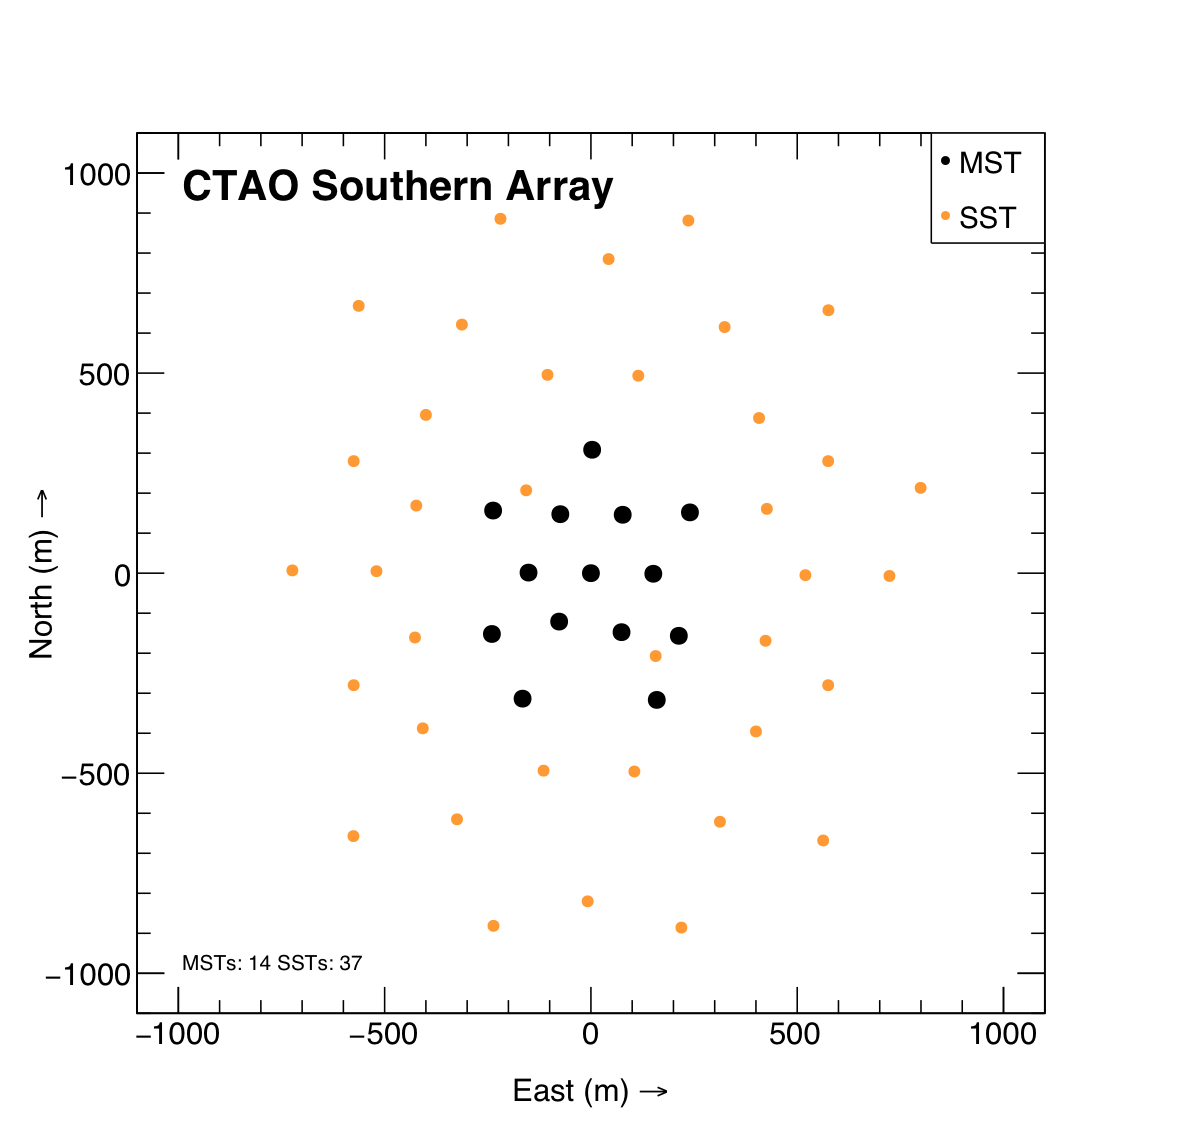
\includegraphics[width=0.7\columnwidth]{figures/southlayout.png}
        % note that in above figure file name, "sr_setup",
        % the file extension is missing. LaTeX is smart enough to find
        % apropriate one (i.e. pdf, png, etc.)
        % You can add this extention yourself as it seen below
        % both notations are correct but above has more flexibility
        %\includegraphics[width=1.0\columnwidth]{sr_setup.pdf}
        \caption{
                \label{fig:southlayout} % spaces are big no-no withing labels
                % things like fig: are optional in the label but it helps
                % to orient yourself when you have multiple figures,
                % equations and tables
                The CTA-South alpha array configuration, taken from \cite{zencta}.
        }
\end{figure}
\subsection{CHEC}
\begin{figure}[ht] 
        % read manual to see what [ht] means and for other possible options
        \centering 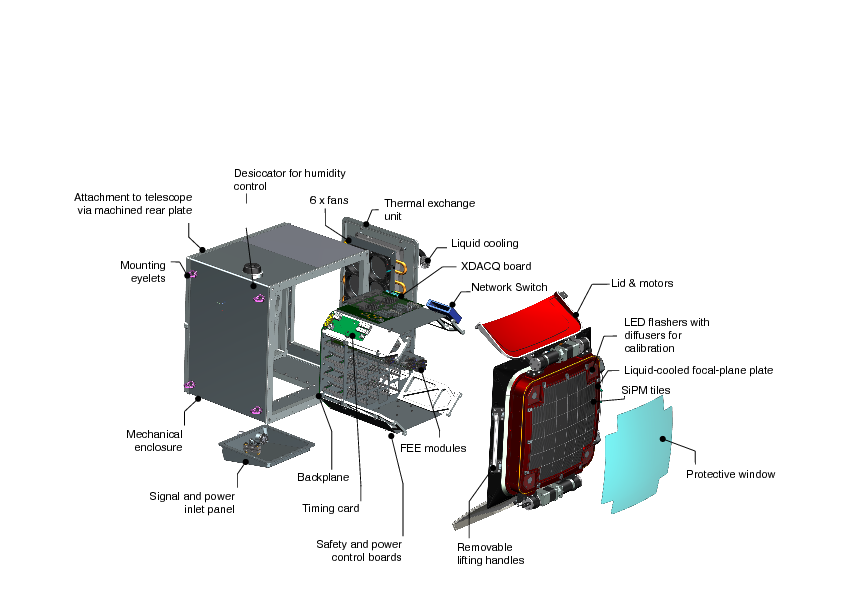
\includegraphics[width=\columnwidth]{figures/cam.png}
        % note that in above figure file name, "sr_setup",
        % the file extension is missing. LaTeX is smart enough to find
        % apropriate one (i.e. pdf, png, etc.)
        % You can add this extention yourself as it seen below
        % both notations are correct but above has more flexibility
        %\includegraphics[width=1.0\columnwidth]{sr_setup.pdf}
        \caption{
                \label{fig:cam} % spaces are big no-no withing labels
                % things like fig: are optional in the label but it helps
                % to orient yourself when you have multiple figures,
                % equations and tables
                The CHEC-S CAD model with key elements highlighted, taken from \cite{rwhite}.
        }
\end{figure}
The UK's main material contribution to CTA construction is planned to be construction of a variant of the Compact High Energy Camera (CHEC), which is designed to work with SST structures that have a dual-mirror (Swartzchild-Couder) optical design. CHEC was designed to be compatible with both the GCT and ASTRI optical structures.  Two operational CHEC prototypes have already been built. The first, CHEC-M, has as its light detectors 32 Multi-Anode Photomultipliers (MAPMs)\cite{tomthesis}. These consist of a block of 8x8 pixels, the signals from which are digitised at a rate of $1\mathrm{GSa}/\mathrm{s}$ \cite{tomthesis} by front end electronics based upon the custom TARGET application-specific integrated circuit (ASIC) \cite{checmpaper}. When it is triggered by two or more four pixel blocks exceeding a discriminator threshold, the data is read out of the camera over a 96ns window containing 96 photoelectron samples. A refined prototype, CHEC-S, is currently undergoing testing at the Max Planck Institute for Nuclear Physics in Heidelberg. CHEC-S contains a refinement of the TARGET-based electronics of its predecessor, but replaces the MAPMs with Silicon Based Photomultipliers (SiPMs). These have the advantage of being more durable than MAPMs, but are also cheaper and can operate in conditions with a higher night sky background (NSB). CHEC is designed to work with SST structures that have a dual-mirror (Swartzschild-Couder) optical design. This design allows for a compact camera (approximately 0.4 m diameter) with small scale photosensors (6/7 mm, corresponding to roughly a third of the plate scale of a comparable single mirror design) and a wide field of view ($\sim$0.2 degrees per pixel). Two operational CHEC prototypes have already been built, the most recent of which (CHEC-S) is currently undergoing testing at the Max Planck Institute for Nuclear Physics in Heidelberg, and has recently been used on an observing campaign on the ASTRI prototype. Further details regarding the science performance of the SST sub-array and the complete CTA instrument can be found in Maier et. al \cite{gernotCTA} and Hassan et. al \cite{tarekCTA}.

Both CHEC cameras and the upcoming SSTCAM have inbuilt self-calibration LED flasher systems, designed to flat-field the camera. The flashers on the CHEC prototypes were attached to the camera corners and reflected off the secondary mirror, for the final SSTCAM design the flasher will most likely be situated behind the secondary mirror and shine through. 

\subsection{GCT, ASTRI and the SST Harmonization Process}

There are two SST dual-mirror prototype designs that CHEC cameras can be attached to, the French led Gamma Cherenkov Telescope (GCT), and the Italian led Astrofisica con Specchi a Tecnologia Replicante Italiana (ASTRI) instrument. Both share a Schwartzchild-Couder optical design, which allows for a compact silicon photomultiplier camera as well as a more uniform Point Spread Function (PSF) across the field of view. Following a harmonisation process, the ASTRI optical design with a CHEC-type camera was selected for the SSTs, taking into account lessons learned from all prototypes. But for the purposes of the results in this thesis which are primarily concerned with the camera, these two optical structures are interchangeable (in Chapter \ref{ch:3-TimingInfo} we consider CHEC-S with GCT as our instrument, whereas in the later  Chapter \ref{ch:5-CHECNSB} we consider CHEC-S on ASTRI). 

\begin{figure}[ht] 
        % read manual to see what [ht] means and for other possible options
        \centering 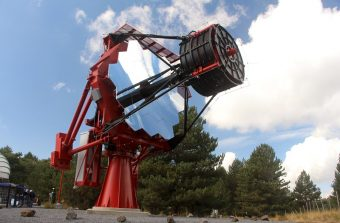
\includegraphics[width=\columnwidth]{figures/astri-horn.jpg}
        % note that in above figure file name, "sr_setup",
        % the file extension is missing. LaTeX is smart enough to find
        % apropriate one (i.e. pdf, png, etc.)
        % You can add this extention yourself as it seen below
        % both notations are correct but above has more flexibility
        %\includegraphics[width=1.0\columnwidth]{sr_setup.pdf}
        \caption{
                \label{fig:astri} % spaces are big no-no withing labels
                % things like fig: are optional in the label but it helps
                % to orient yourself when you have multiple figures,
                % equations and tables
                The ASTRI-Horn prototype on Sicily. Image Credit: CTA Collaboration.
        }
\end{figure}

\section{Methods and Environments of Astrophysical $\gamma$-ray Emission}
\subsection{Inverse Compton Scattering}

Inverse Compton scattering describes the process by which low energy photons are scattered by ultra-relativistic electrons, significantly increasing the kinetic energy of the photons. The photon fields accelerated by the electrons vary; they can be a population of photons produced through synchrotron emission that are then hit by the high energy electrons that emitted them (so-called synchrotron self-Compton emission), can be the result of starlight, or originate from the cosmic microwave background. In the rest frame of the electron, the ratio of final photon energy over initial energy is given by
\begin{equation}
    \frac{E_f}{E_i}=\gamma (1+\beta \cos(\theta))
\end{equation}
where $\gamma$is the Lorentz factor of the electrons and $\theta$ is the deflection angle. Transferring to the observer frame this works out at around $\frac{E_f}{E_i}\sim \gamma^2$. This results in the spectral emissivity from inverse Compton scattering of an isotropic photon field of single photon frequency $v_0$ by a power law distribution of electrons being given by 
\begin{equation}
    I(v)dv=\frac{3\sigma_TcvN(v_0)}{16\gamma^4v_0^2}\left(2c\ln\left(\frac{v}{4\gamma^2v_0}\right)+v+4\gamma^2v_0-\frac{v^2}{2\gamma^2v_0}\right)dv
\end{equation}
where $N(v_0)$ is the number density of photons, $\sigma_T$ is the Thompson cross section, $v$ is the frequency of the $\gamma$-rays \cite{blumenthal}.


\subsection{Hadronic Emission}
The collision of two sufficiently high energy protons can create pions through strong interactions.  A typical interaction scheme \cite{EAS} is
\begin{gather*}
\mathrm{p}+\mathrm{p}\rightarrow \mathrm{N}+\mathrm{N}+n_1 \mathrm{\pi^{\pm}}+n_2\mathrm{\pi^0} \\
\mathrm{\pi^0} \rightarrow \mathrm{2\gamma} \\
\mathrm{\mathrm{\pi^{\pm}}} \rightarrow \mathrm{\mu^{\pm}}+\mathrm{\overset{(-)}{\nu_{\mu}}}\\
\mathrm{\mu^{\pm}} \rightarrow \mathrm{e^{\pm}}+\mathrm{\overset{(-)}{\nu_{\mu}}}+\mathrm{\overset{(-)}{\nu_{e}}}
\end{gather*}
where $N$ represents the resulting fragmented hadrons which are produced along with $n_1$ charged pions and $n_2$ neutral pions. The charged pions have a lifetime of which have a short lifetime of only 26 ns, but the neutral pions' lifetime is much shorter at $5 \times 10^{-17} \mathrm{s}$ because it decays due to the electromagnetic force. Hadronic emission processes are challenging to discriminate from inverse Compton scattering in some sources, particularly supernova remnants \cite{rxjcta}. The recent detection of an astrophysical neutrino (IceCube-170922A) by IceCube that was coincident with a $\gamma$-ray flare of the blazar TXS 0506+056 suggests that some $\gamma$-rays from blazars are produced by hadronic processes, likely close to the associated supermassive black hole \cite{TXS}. As we'll see later in this chapter, these fundamental processes occur in the same way in EAS, when a high energy cosmic ray hits the Earth's atmosphere.

\subsection{Known Astrophysical $\gamma$-ray Sources}
$\gamma$-rays are known to be produced by hadronic and inverse compton processes in a variety of environments. These include supernova remnants, Active Galactic Nuclei (AGN, typically blazars where the jet of the AGN points towards Earth), pulsar wind nebulae, $gamma$-ray binaries \cite{scienceCTA} and most recently Novae [H.E.S.S., in prep]. Gamma-ray bursts have also recently been observed by IACTs on the ground for the first time \cite{magicGRB}; these can originate from neutron star collisions or supernovae. There is also both galactic and extragalactic diffuse $\gamma$-ray emission seen by IACTs. In the galactic case it is believed the majority of the emission results from hadronic emission due to collisions of cosmic rays with galactic gas \cite{extragamma}. The extragalactic case is less well understood \cite{extragamma}, with the majority of emission likely due to unresolved blazars, radio galaxies and star-forming galaxies, but some additional components may be due to dark matter annihilation or cosmic ray interactions.

\section{The Key Science Projects of CTA}
The CTA observing time not allocated to open observations will be dedicated to a number of Key Science Projects (KSPs). In this section we briefly explore the science potential for each of these missions.

\subsection{The Galactic Centre KSP}
CTA observations will be made of the central square degree of the Milky Way for 500 hours \cite{scienceCTA}, with a further 300 hours spent observing the region up to 10 degrees in galactic latitude. It is anticipated that this will be one of the first major campaigns for CTA due to its implications for other CTA surveys.
In particular, the galactic centre is considered one of the best places to search for evidence of dark matter annihilation, and these observations should be sufficient to obtain either a detection or an upper limit for many of the current best dark matter models \cite{scienceCTA}. Additionally, these observations hope to uncover the nature of the galactic centre gamma-ray source, and to probe the nature of very high energy particle acceleration in the galactic centre (key to understanding the nature of the Fermi Bubbles as explored in Section 6). 

\subsection{The Galactic Plane Survey (GPS) and the Cosmic Ray PeVatron KSP}
Around 1800 total hours of observing time will be spent performing observations of the galactic plane, with a sensitivity of at least 4.2 mCrab \cite{scienceCTA} (an improvement of 5-20 times relative to current instruments). It is planned that this survey will lead to the discovery of new galactic sources of TeV gamma rays, including supernova remnants, gamma-ray binaries and Pulsar Wind Nebulae. Additionally, it will provide new constraints for models of the galactic diffuse emission and source populations. 

It is anticipated that the maps generated by the GPS will be periodically made public, in order to maximize its multi-wavelength science potential.
Additionally, the PeVatron KSP aims to perform dedicated, deep observations of known gamma-ray sources with particularly hard spectra (such as RX J1713.7-3946), and search for diffuse gamma-ray emission around known Supernova Remnants in an attempt to understand the origins and acceleration methods of cosmic rays \cite{scienceCTA}.

\subsection{The Large Magellanic Cloud Survey and the Star Forming Systems KSP} Around 600 hours of CTA observation time will be spent on observing the Large Magellanic Cloud (LMC). In particular, the LMC is interesting at TeV energies due to its high rate of star formation; the LMC produces about one tenth of the number of stars as the Milky Way, but has only 2\% of the Milky Way's volume \cite{scienceCTA}.
As such, it contains a disproportionate number of supernova remnants (such as SN1987A) and pulsar wind nebulae.  These can be observed more easily in the LMC than in the Milky Way due to the absence of source confusion, interstellar absorption and line of sight crowding at the LMC's high galactic latitude \cite{scienceCTA}. Other observations of galactic star forming regions (for example Westerlund 1) are also planned as part of the star forming systems KSP, in order to investigate the link between star formation and particle acceleration.

\subsection{The Extra-Galactic Survey and the AGN KSP} One of the largest time allocations, the extra-galactic survey will cover 25\% of the sky down to 6 mCrab sensitivity \cite{scienceCTA}. It will aim to achieve an unbiased census of gamma-ray AGN, observe fast-flaring sources and gamma-ray busts serendipitously, and measure the anisotropies in the electron cosmic ray spectrum. Key to this is CTA's ability to operate in a divergent pointing mode, where not all telescopes in the array are pointing at the same patch on the sky. 

An AGN KSP is also envisaged to perform long term monitoring of a select set of Active Galactic Nuclei, in order to understand how the different types of AGN are related, and how their particle and gamma-ray acceleration mechanisms work \cite{scienceCTA}. By extension, these observations should also act as a probe of the intergalactic magnetic field and the extragalactic background light. The AGN KSP is also a means of performing tests of fundamental physics, and CTA should be able to place constraints on Lorentz Invariance Violation and the production of Axion-like particles through the monitoring of AGN. 

\subsection{The Transient KSP} Somewhat intertwined with the Extra-Galactic Survey, CTA will have the capability to respond to transient events from both internal and external triggers. These external triggers will be sent by Gravitational Wave, Neutrino, Radio, Optical, X-ray and Gamma-ray observatories around the world when they detect a transient object. Following such a trigger, CTA will immediately perform follow-up observations to help constrain the emitting object's nature \cite{scienceCTA}. Likewise notifications of transient events serendipitously detected by CTA will be sent to partner observatories.

\section{Types of IACT Backgrounds}
\subsection{Hadronic Air Showers}

In order to perform all of the scientific investigations explored in Chapters \ref{ch:3-TimingInfo} and \ref{ch:4-VERITASRealData}, along with the guest observation program, we need to be able to distinguish astrophysical gamma-ray signals from background reliably. Unfortunately, not all EAS are caused by gamma-ray photons. For most energies, EAS caused by incident charged hadrons (most commonly protons) outnumber those caused by photons by a factor of roughly 10,000 \cite{Benbow}. These provide a significant background to IACTs, and are the largest constraint on their sensitivity.

\begin{figure}
\begin{center}  

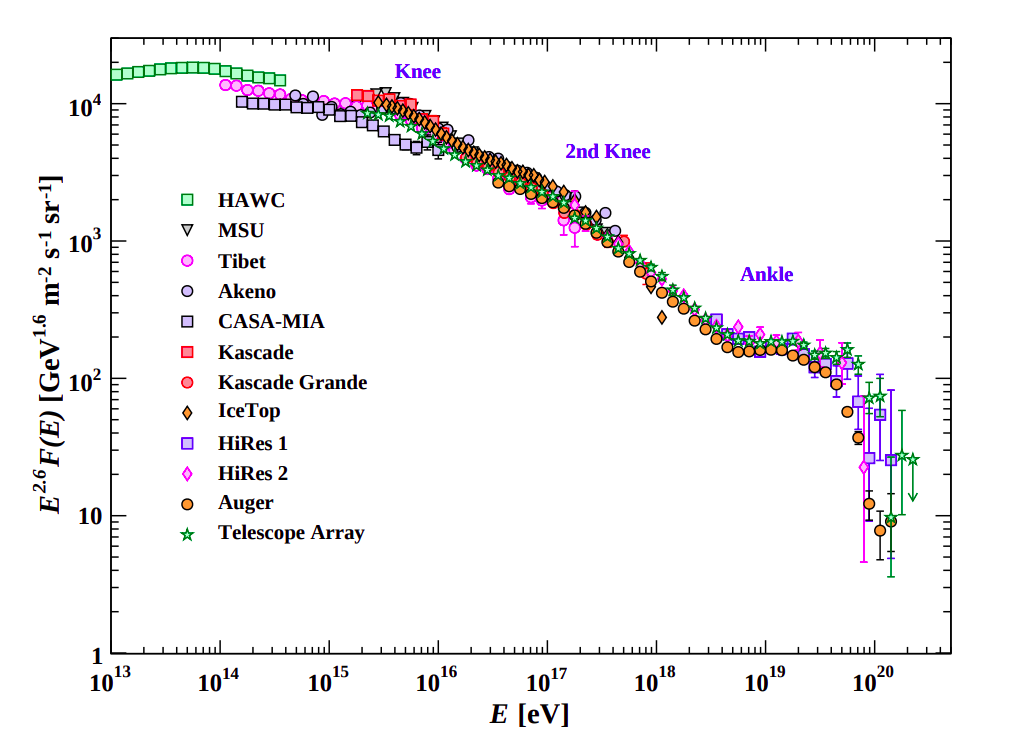
\includegraphics[width=\columnwidth]{figures/pdgcr.png}
 
\caption{The all particle cosmic ray spectrum, taken from \cite{pdg}. Whilst mainly protons, this spectrum includes both cosmic ray electrons and heavier element cosmic rays. The spectrum is a power law with index -2.7 up to around $3 \times 10^6$ GeV, where it steepens to an index of -3.1, a transition feature known as 'the knee'. It then flattens back to an index of -2.7 at $4 \times 10^9$ GeV (a feature known as 'the ankle'. The lower energy cosmic rays below the knee are believed to be galactic in origin, most likely a result of acceleration in supernova remnants. The higher energy cosmic rays above the knee are believed to be the result of cosmic ray acceleration in extragalactic sources such as Active Galactic Nuclei (AGN). The so-called GZK cutoff is theorised to exist at energies around 50 EeV \cite{gzk}, the limit at which a cosmic ray could propagate from another galaxy without interacting with the CMB. For comparison, the LHC operates at a centre of mass energy of 14TeV for proton-proton collisions, corresponding to an initial EAS proton energy of $1\times 10^{17}$eV.}
\label{fig:crspec}
\end{center}
\end{figure}

However, because the quarks contained within protons experience the strong nuclear force, the typical interactions they undergo on entering the atmosphere are different to photons, the typical products of these interactions are photons, muons and electrons. The rest frame lifetime of the muons is only 2.197 $\mu$s \cite{pdg}, however because the muons produced in these interactions are highly relativistic, the muons can survive to ground level as a results of time dilation effects, but some decay to electrons via the weak nuclear force. The muons also undergo a significant number of inelastic scattering interactions, carrying a larger fraction of the total transverse momentum away from the shower core and resulting in a wider overall EAS compared to a gamma-ray induced shower \cite{tomthesis}.  The resultant $\gamma$-rays from $\pi_0$ decay (as seen earlier in this chapter) can themselves undergo pair production creating electromagnetic sub-showers of the hadronic shower core. The charged products are typically highly relativistic and thus produce detectable Cherenkov light.  Whilst the interaction scheme for hadronic air showers is more complex than for $\gamma$-ray or electron induced ones, it is still possible to construct semi-analytic models of their evolution. The most notable of these is the Heitler-Matthew model, details regarding this can be found in \cite{heitler}.

%Not all background for Cherenkov telescopes can be attributed to Cherenkov light, atomic oxygen, hydroxide and sodium airglow emission lines in the atmosphere can contribute significantly at sufficiently long wavelength \cite{pmtubes}. However, we neglect this effect in this report as it can be negated by operating at short wavelengths and operating from a dark enough site.

\begin{figure}
\begin{center}  

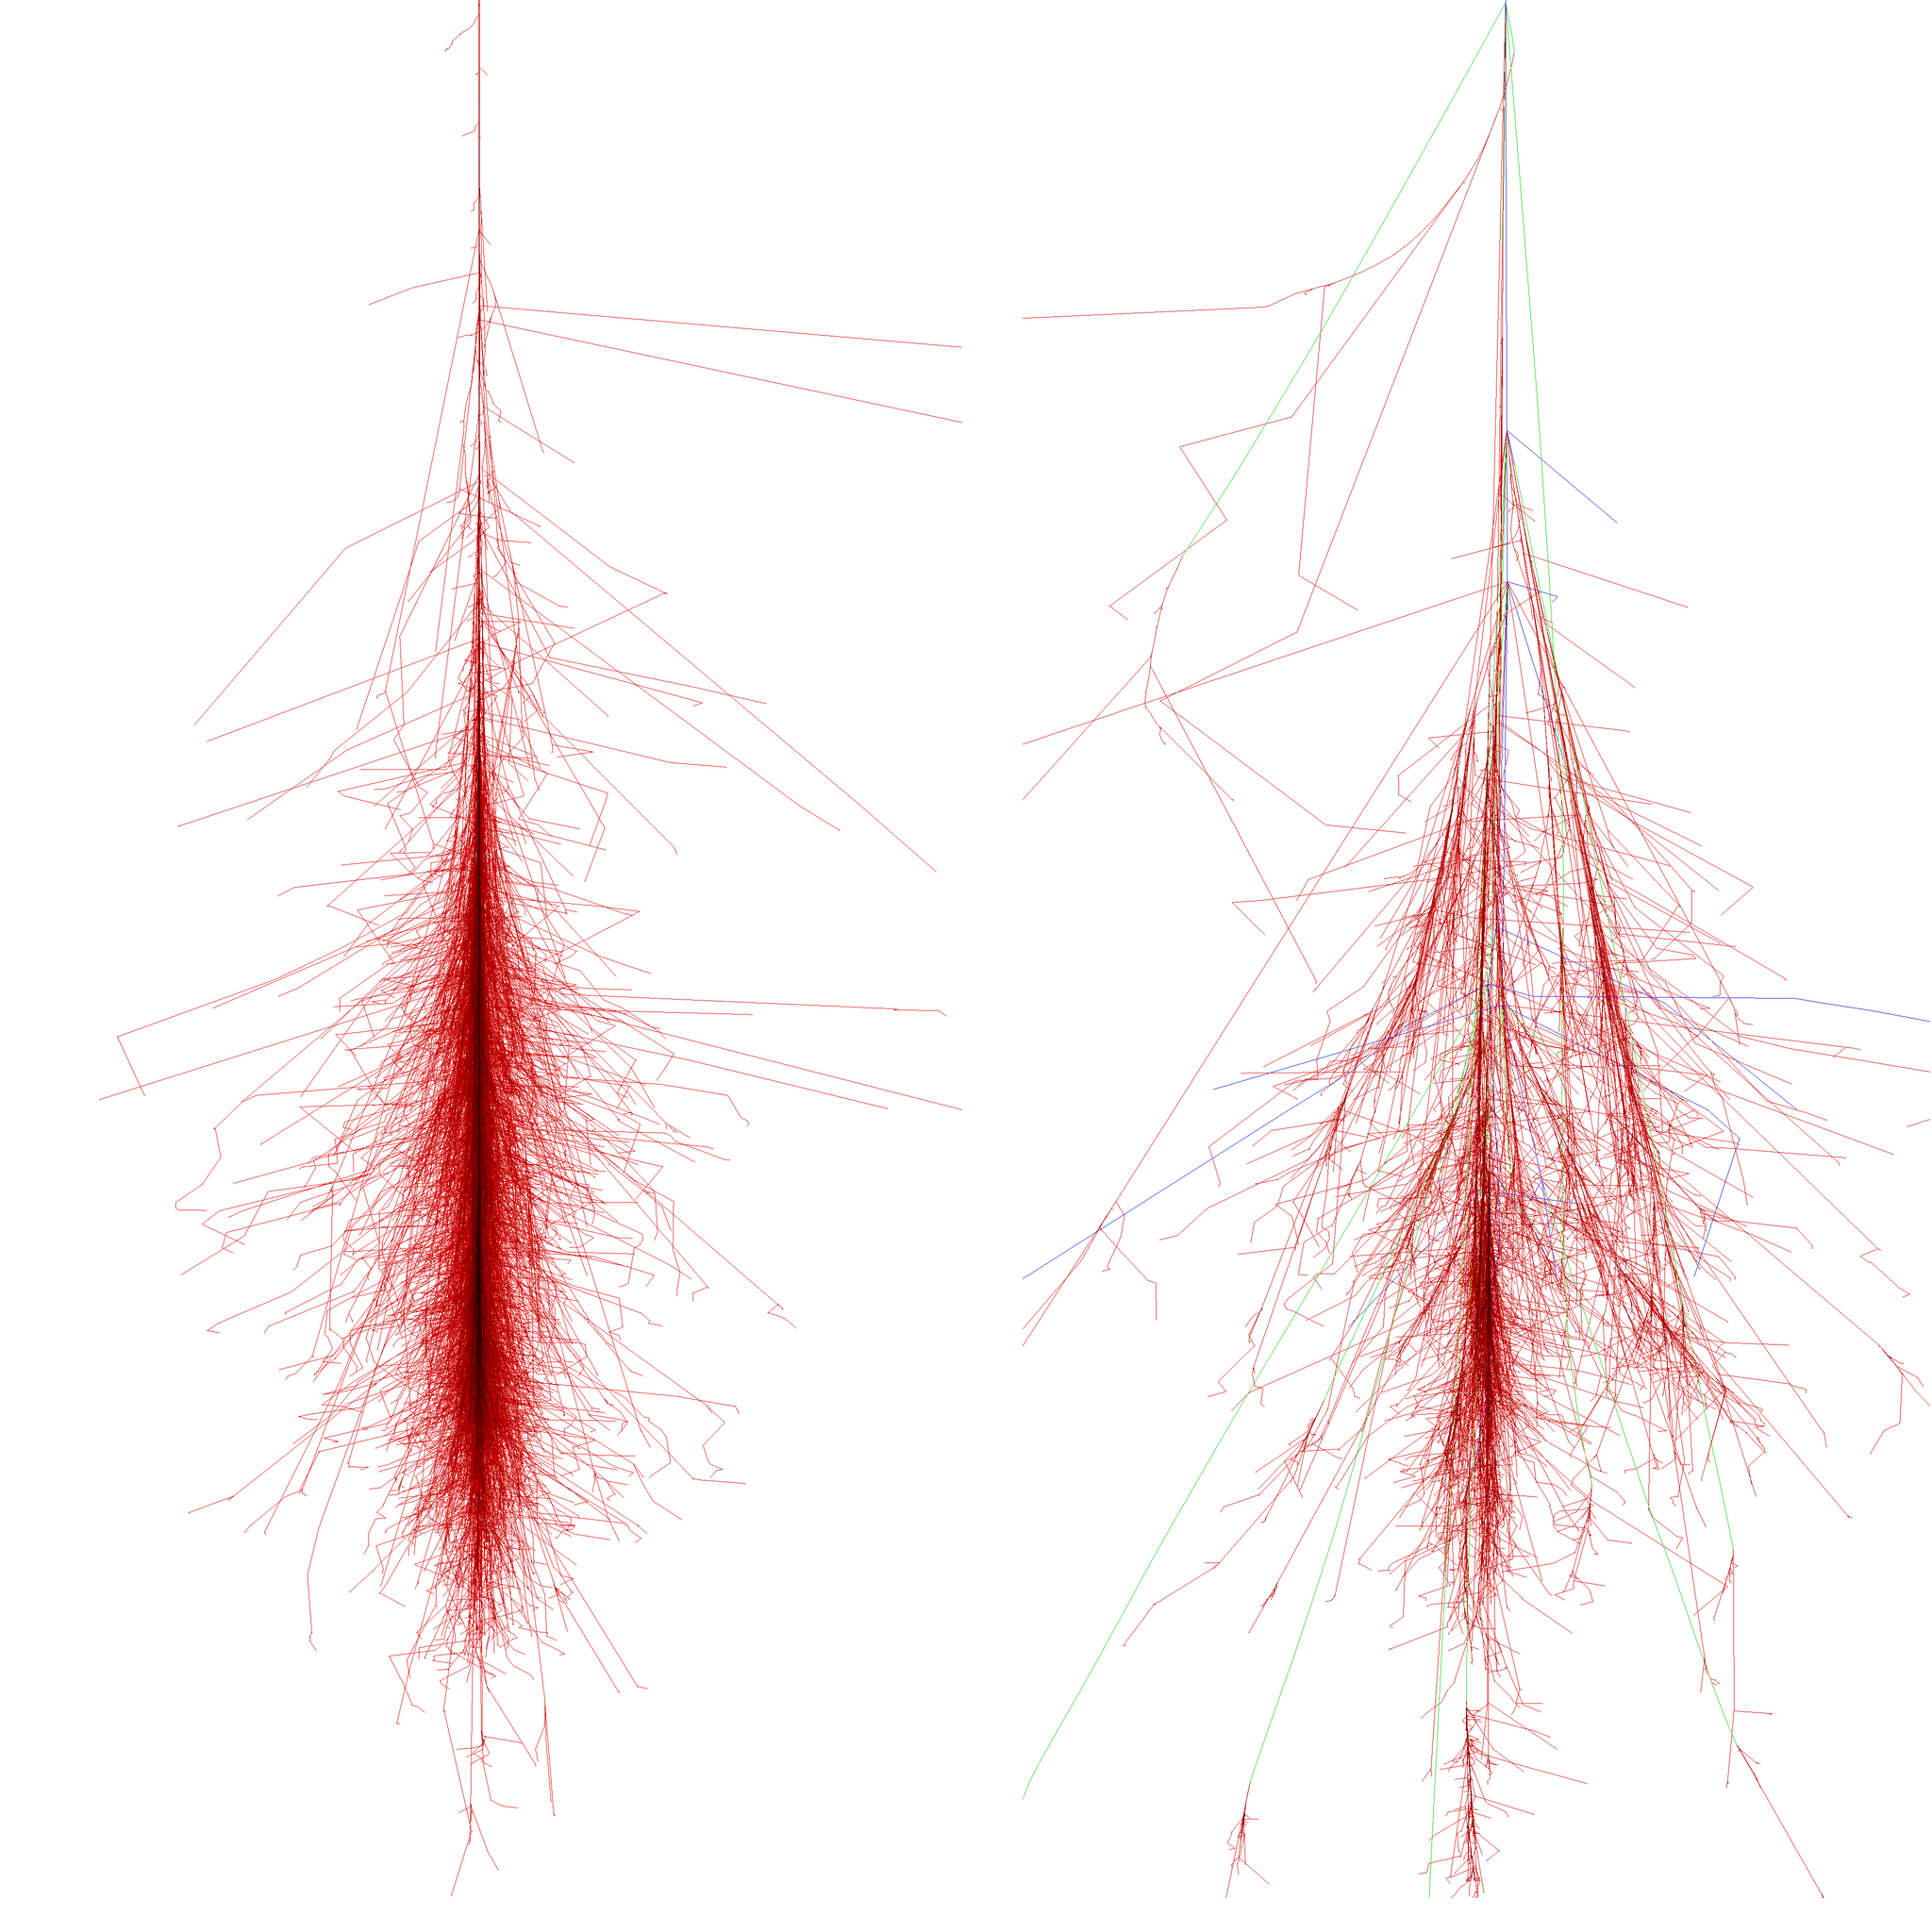
\includegraphics[width=0.5\columnwidth,trim=4 4 30 4,clip]{figures/showers.png}
 
\caption{XZ plots of CORSIKA simulations of particle tracks for 100 GeV photon (left) and proton (right) events. Note the wider, less concentrated proton shower (taken from \cite{corskplot}).}
\label{fig:image2}
\end{center}
\end{figure}
\subsection{Electron Air Showers}

Electrons can also be a significant source of background at low TeV energies as they are difficult to distinguish from $\gamma$-rays and undergo similar interactions. There are two small differences between electron and $\gamma$-induced air showers. The first is the process by which the primary particles interact on hitting the atmosphere, a primary $\gamma$-ray will typically loose all its energy in a single pair production event, whereby a primary electron of the same initial energy can loose energy via production of numerous lower-energy Bremsstrahlung photons which can create electromagnetic sub-showers. This can create a relatively greater number of Cherenkov photons at higher altitudes for electron-induced showers. The other small difference between the two is the average altitudes at which they first interact \cite{Sitarek1i}, which is due to the radiative length of an electron being smaller than the pair production length of a $\gamma$-ray. As a result, a primary cosmic-ray electron of the same energy as a primary $\gamma$-ray will begin interacting higher in the atmosphere, resulting in a higher-altitude shower maximum \cite{lypova}. 

\subsection{Night Sky Background}
Night Sky Background (NSB), which refers to the light detected in Cherenkov camera images that is not attributable to Cherenkov light, is complex and in general, poorly modelled and understood. It consists of photons from a variety of sources (including, but not limited to)

\begin{itemize}
    \item Atmospheric Air glow emission lines, particularly from atomic oxygen, hydroxide and sodium.
    \item Moonlight
    \item Stars
    \item Zodiacal light, along with diffuse galactic light and extragalactic background light (though these contributions are small). \cite{nsbref}
    \item Light Pollution from Population Centres
\end{itemize}

Historically, analytic studies of NSB have been limited, as the standard CORSIKA and sim\_telarray simulation packages do not attempt to model NSB in a particularly realistic way. Most previous work on NSB has focused on direct observations with photomultipliers \cite{BandE}. 

\section{Standard IACT Stages of Event Analysis}\label{app:imaging}

\subsection{Trigger Selection}

Trigger selection is a feature of an IACT array designed to automatically reject events with a low probability of being astrophysical gamma-rays in the readouts of the camera. CHEC-S, for example, only reads out the camera photomultipliers if two adjacent superpixels (blocks of four adjacent pixels) passes a comparator check. The VERITAS trigger is slightly more complex, it consists of a single pixel trigger which acts on individual pixels (and includes timing analysis), a camera level trigger which works on the pattern and relative timing of the single pixel triggers, and an array trigger which requires that more than two telescopes are triggered in order such that an event is stored to disk\cite{veritastrigger}. This array-level trigger in particular significantly reduces the number of false triggers associated with muons passing through the instrument and telescope optics, as it is unlikely a single cosmic ray muon will generate sufficient Cherenkov light to trigger a second VERITAS telescope a few tens of meters away. A combination of trigger selection and simple parameter-based cuts can reduce the signal to background ratio to 1:1 for a bright source like the Crab Nebula using a current generation instrument like H.E.S.S. \cite{Berge07}.

\subsection{Pedestal Subtraction/Calibration}

Electronic noise present in IACT camera data needs to be removed. For this purpose, measurements of the camera noise are taken when the camera is shut off from the outside environent with the shutter closed (similar to dark framing for optical astronomy). These measured pedestals are then subtracted from the observed live data.

\subsection{Charge Integration}

Charge integration is the process of taking a calibrated PMT trace and extracting the number of photoelectrons. Various schemes exist for performing this operation, CHEC/SSTCAM relies on a cross-correlation template fitting model developed by J. Watson \cite{jasonthesis}.

\subsection{Tailcut Cleaning}

Before conventional IACT analysis, the sensitivity of event classification and reconstruction to features in images from NSB requires that the images from the Cherenkov cameras are cleaned. The conventional method of doing this is tailcut cleaning with two thresholds, whereby a pixel is only included in the analysis if the number of photoelectrons in the pixel exceeds a given threshold, or if it is the neighbour of such a pixel and also has a greater number of photoelectrons than a (typically lower) second threshold \cite{hegratailcut}. These thresholds require optimisation to achieve a desired event rate, and the implementations of this procedure vary by instrument (see for example \cite{magictailcut}\cite{Benbow}\cite{magictime}). Alternatively methods based upon wavelet image cleaning have been proposed \cite{wavelet}, but these are far more rarely used in practice. One of the aims of deep learning based image analyses that we explore in Chapters \ref{ch:3-TimingInfo} and \ref{ch:4-VERITASRealData} is to avoid this tailcut cleaning step, as some light from the Cherenkov shower itself is sometimes lost, however previous attempts at performing deep learning without requiring this step have failed when the event classifier or reconstruction method is exposed to real data. 

\subsection{Hillas Parameter Based Techniques for Event Classification}
\begin{figure}[ht] 
        % read manual to see what [ht] means and for other possible options
        \centering 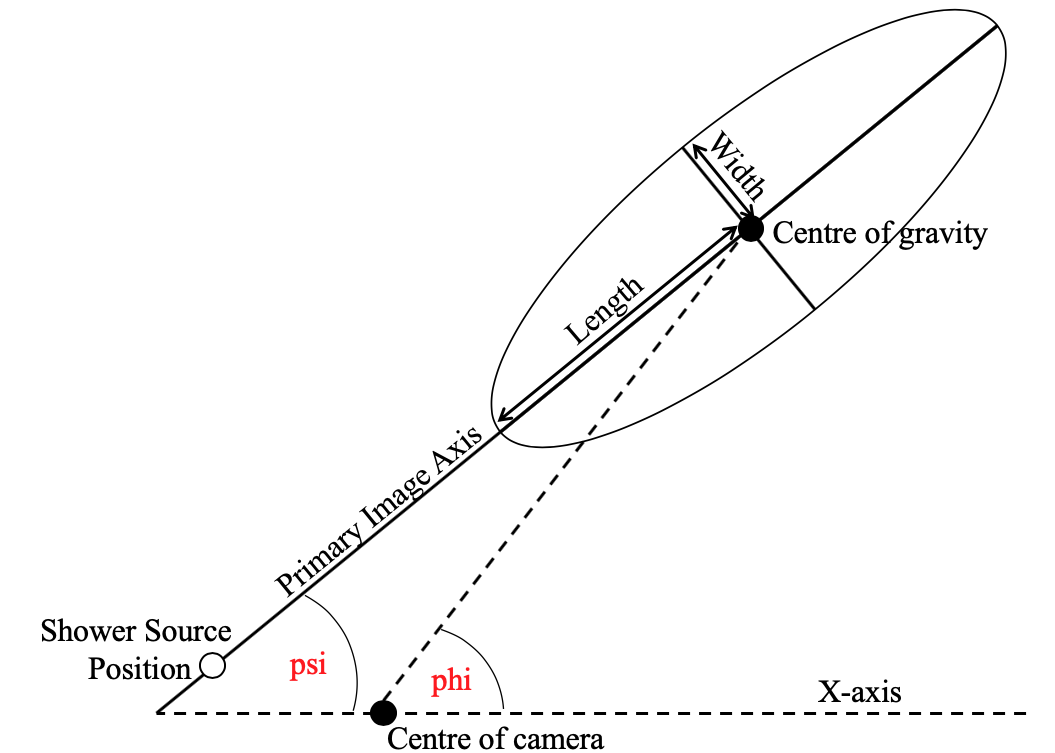
\includegraphics[width=\columnwidth]{figures/hillas.png}
        % note that in above figure file name, "sr_setup",
        % the file extension is missing. LaTeX is smart enough to find
        % apropriate one (i.e. pdf, png, etc.)
        % You can add this extention yourself as it seen below
        % both notations are correct but above has more flexibility
        %\includegraphics[width=1.0\columnwidth]{sr_setup.pdf}
        \caption{
                \label{fig:hillas} % spaces are big no-no withing labels
                % things like fig: are optional in the label but it helps
                % to orient yourself when you have multiple figures,
                % equations and tables
                The definition of Hillas parameters, taken from \cite{ctapipe}.
        }
\end{figure}
Hillas Parameters form the basis of the methods for event discrimination in the current generation of IACTs, and were instrumental in obtaining the first reliable gamma-ray source detection of the Crab nebula from the ground \cite{whipple} (much of the previous work in the years following 1953 centred on Pulsar detection and has since largely been disproved \cite{paulathesis}). They are obtained \cite{tomthesis} \cite{weekestev} from the second moments of an IACT camera image (constructed from the total integrated charge for each photomultiplier pixel), defined as 
\begin{align*}
\langle x^2 \rangle = \frac{\sum_i I_i x_i^2}{\sum_i I_i} && \langle y^2 \rangle = \frac{\sum_i I_i y_i^2}{\sum_i I_i}
\end{align*}
where $x_i$ and $y_i$ are the pixel co-ordinates and $I_i$ the associated pixel intensity. From these and the expectation values of $x$ and $y$ one can construct the variance and covariance
\begin{align*}
\sigma_x^2=\langle x^2 \rangle - \langle x \rangle^2&&\sigma_y^2=\langle y^2 \rangle - \langle y \rangle^2&&\sigma_{xy}=\langle xy \rangle - \langle x \rangle\langle y \rangle
\end{align*}
and define the following quantities
\begin{align*}
d=\sigma_x^2-\sigma_y^2&&a=(d+\sqrt{d^2+4\sigma_{xy}^2})/2\sigma_{xy}.
\end{align*}
The Hillas Parameters relevant for event classification are the width and length of the ellipse which characterize the transverse and lateral development of the shower and are defined by
\begin{align*}
W=\sqrt{\frac{\sigma_y^2+a^2\sigma_x^2+2a\sigma_{xy}}{1+a^2}}&&L=\sqrt{\frac{\sigma_x^2+a^2\sigma_y^2+2a\sigma_{xy}}{1+a^2}}.
\end{align*}
In order to take into account information from all of the telescopes in the array, these parameters must be combined into the Mean Reduced Scaled Width and Length (MRSW/MRSL), defined by a sum over all telescopes such that
\begin{align*}
SW&=\frac{W-\langle W \rangle}{\sigma_W}   &    SL&=\frac{L-\langle L \rangle}{\sigma_L}\\
\\ MRSW&=\frac{1}{\sum \omega}\sum SW\cdot \omega & MRSL&=\frac{1}{\sum \omega}\sum SL\cdot \omega
\end{align*}
where $\sigma_W$ is the spread of the expected width which must be obtained from Monte-Carlo generated lookup tables and $\omega=\langle W \rangle^2/\sigma_W^2$ is a weighting factor to take into account these tables' accuracy.

Initially Hillas Parameters were simply used to perform data cuts to separate hadronic showers from gamma-ray induced showers based on their differing morphology. However in recent years, more sophisticated methods using Boosted Decision Trees (BDTs) (taking the MRSL, MRSW, total integrated charge and other parameters derived from Monte-Carlo lookup tables) eventually became the preferred methods for incident particle classification \cite{hessbdt}.

Hillas parameter based techniques don't however take advantage of the full camera image of the EAS, and as such, subtle details (such as hadronic `halos' \cite{model++}) in the images are not taken into account. This becomes an issue at the sensitivity boundaries that CTA is aiming to considerably improve (particularly in the case of weak or very extended sources), as hadronic and electron induced showers can closely resemble those generated by gamma-rays. This motivates us to investigate new analysis techniques for event discrimination in order to improve the IACT sensitivity.

\begin{figure}[ht] 
        % read manual to see what [ht] means and for other possible options
        \centering 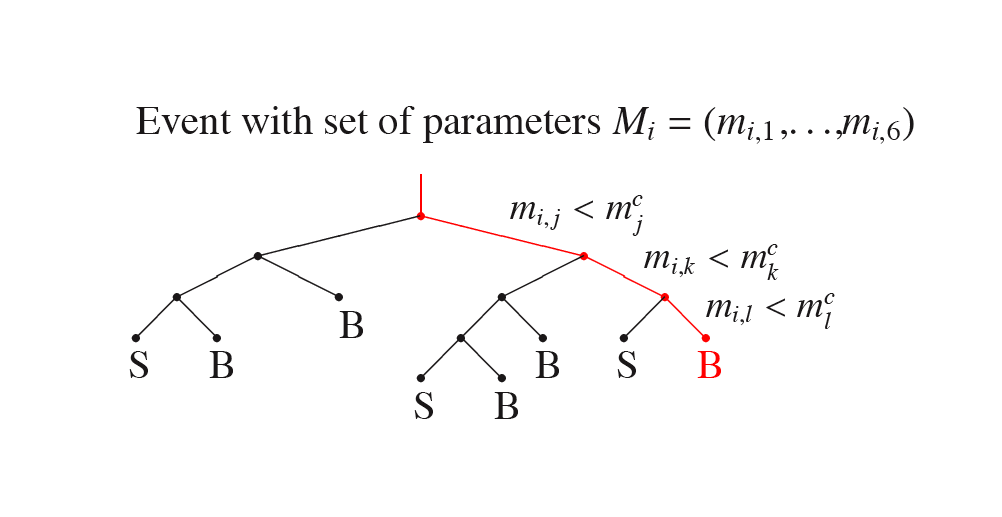
\includegraphics[width=\columnwidth]{figures/forest_picture.png}
        % note that in above figure file name, "sr_setup",
        % the file extension is missing. LaTeX is smart enough to find
        % apropriate one (i.e. pdf, png, etc.)
        % You can add this extention yourself as it seen below
        % both notations are correct but above has more flexibility
        %\includegraphics[width=1.0\columnwidth]{sr_setup.pdf}
        \caption{
                \label{fig:network} % spaces are big no-no withing labels
                % things like fig: are optional in the label but it helps
                % to orient yourself when you have multiple figures,
                % equations and tables
                An example of a BDT, taken from \cite{hessbdt}. The event is classified as either Signal (S) or Background (B) by the tree based on whether at each node on the tree the parameters $m_{i,j}$ are larger than the weights $M^c=(m^c_j,...)$. The ultimate event classification is not performed by one tree, but by the weighted mean of an ensemble of trees generated iteratively by evaluating the trees' efficiency against training data.
        }
\end{figure}

\subsection{Event Selection Cuts and Run Selection}

IACT observations are normally conducted in runs, where the IACT array tracks and observes a single source. The length of these runs varies, but most IACT observatories use between 20 and 30 minutes. This is as to obtain a sufficient number of events to accurately model background, whilst observation conditions are roughly constant.

Most IACT analysis begins with Hillas parameter cuts on the data to remove obviously hadronic events (with very high MRSW) and events far from the desired source (so-called theta squared cuts).
It is also common to remove runs or events from an IACT analysis for a variety of reasons. The data from a run may be low quality due to poor weather conditions, hardware or tracking issues or high zenith angle (where simulation accuracy drops due to the complexity of modelling the atmosphere correctly). Most IACT analyses use multiple runs per source, though the work in Chapter \ref{ch:4-VERITASRealData} considers only a single VERITAS run as we attempt to match the data more closely.

\subsection{ON/OFF Region and Reflected Region Analysis}
So far we have focused on Cherenkov camera based background rejection, however this only reduces the signal to background rate (by around a factor of 100) to ~1:1 for bright sources. As such, there is a need for a higher level background rejection method, similar to aperture photometry in optical astronomy. The simplest method possible is to take one ON region and one OFF region at the same right ascension but differing declination. The disadvantage of this is the loss of time on source. An alternative developed by the Whipple observatory is so called 'Wobble Mode', where the telescope wobbles around the source in declination, allowing for more time on source. However, this is complicated by two factors, the comparatively poor angular resolution of IACTs, and the significant extension of some sources such as the supernova remnant RXJ 1713.7-3946. As such, the HEGRA collaboration \cite{HEGRA} developed so called reflected-region analysis, where multiple non-overlapping OFF regions (at different distances from the ON region but of the same angular size) are used. This allows for better statistics compared to a singular OFF region and allows for measurement of a potentially non-uniform night sky background across the field. 

\subsection{CTA Data Analysis Levels}

The proposed CTA analysis pipeline consists of a number of data analysis levels, only some of which are relevant for deep learning analyses. These consist of \cite{jasonthesis}:
\begin{itemize}
    \item r0 data, which is the uncalibrated raw data generated by the Cherenkov camera.
    \item r1 data, which is online, calibrated camera data, calibrated using a scheme specific to the camera.
    \item dl0 data, which is calibrated waveform data along with event metadata, and is zero suppressed to save bandwidth and storage space.
    \item dl1 data, which consists of extracted charge and peak time information extracted from the calibrated waveforms, as well as Hillas parameters extracted from them.
    \item dl2 data, at this stage the telescope multiplicity is dropped and the overall events are characterised (based on their Hillas parameters extracted during the dl1 stage) into 
    \item dl3 data, at this stage the dl2 events are sorted into sets of (for example) $\gamma$-ray candidates. This also includes any relevant instrument response data needed for higher level analysis.
    \item dl4 data, which consists of fully processed event lists, ready for high level astronomical analysis.
    \item dl5 data, which consists of high level analysis data products produced from astronomical analysis, such as the CTA galactic plane survey.
\end{itemize}

The CTA analysis chain will therefore massively reduce the raw amount of data from the telescopes to data scales tractable with a laptop.


\section{Alternatives to Hillas-Parameter-Based Techniques}

\subsection{Template Analyses and Model++}
Template analyses \cite{cat}\cite{3danalysis}\cite{model++}\cite{impact}, which benefit from the fine pixellisation of IACT cameras, form the current main alternative to Hillas parameterisation. They rely on the generation of a library of template IACT images, constructed using either full Monte-Carlo simulations or semi-analytic models. The images from the IACTs are then compared to the templates via a pixel-by-pixel minimisation process, such that the template most resembling the IACT image can be found and thus the shower properties inferred. In particular, such techniques have been commonly applied for directional reconstruction (such as ImPACT \cite{impact}), although the H.E.S.S. Model++ analysis chain uses fitting against semi-analytic models of gamma-ray showers as a background rejection method \cite{model++}.

Whilst Model++ may be widely used within H.E.S.S., the reality that the authors of Model++ have chosen not to make their code open source means that it is not currently seriously being considered as an analysis method for CTA, and its efficacy in the SST energy range has also not been tested. At the time of writing there is no serious effort within CTA to recreate it or to test its applicability in the SST energy range.

\subsection{ImPACT}
The most widely used alternative to Hillas-type analysis is using the Image Pixelwise fit for Atmospheric Cherenkov Telescopes (ImPACT) code \cite{impact}. This works by comparing the shower images to interpolated templates generated using Monte-Carlo simulations. ImPACT was developed for the (previously unprecedentally large) H.E.S.S. II telescope as Hillas parameter based techniques are known to be unreliable at photon energies lower than $50\rm{Ge}V$.  The reconstructed event parameters are the combination of shower parameters for the template which minimizes the total negative log likelihood $\ln\mathcal{L}=\sum_{pixel,i}-2\ln{P(s_i|\mu,\sigma_p,\sigma_y)}$(maximizes the likelihood) over every pixel in the camera for every telescope in the array, where
\begin{equation}
P(s_i|\mu,\sigma_p,\sigma_y)=\sum_n \frac{\mu^n e^{-\mu}}{n!\sqrt{2\pi (\sigma_p^2+n\sigma_{\gamma}^2)}} \exp \left(-\frac{(s-n)^2}{2(\sigma_p^2 + n \sigma_{\gamma}^2)} \right)
\end{equation}
$n$ is the photoelectron number, $\sigma_p$ is the pedestal width (the width of the charge distribution under pure noise), $\sigma_{\gamma}$ represents the photomultiplier resolution, $s$ is the number of signal photoelectrons detected and $\mu$ is the predicted number of photoelectrons from the template. In Practice, ImPACT is only used for directional and energy reconstruction in H.E.S.S. due to concerns about its sensitivity to NSB photons (a problem similar to the real data problem experienced by Convolutional Neural Network (CNN)-type methods). The H.E.S.S. ImPACT chain uses a BDT based on Hillas Parameters for gamma/hadron separation.

The difficulty in using ImPACT for CTA is the requirement of having a sufficient number of template simulations to cope with every possible type of event with a given energy and incident direction for so many telescopes, and the computational cost of searching through those simulations to find the optimal event parameters.

\section{The Prototype CTA Analysis Chain and ctapipe}

CTA is an instrument that is currently in the development phase, and this is true both of the instruments and the analysis pipelines that go with them. For much of the writing of this thesis a full, pythonic analysis pipeline for CTA did not exist, and CTA analyses were a complex mixture of modern code and software written for previous instruments. Additionally, a detailed, complex Monte-Carlo validation procedure was underway relating to the simulated data for even the prototype cameras.

ctapipe is a tool developed as an open-source prototype (which follows modern code practices for version control and code development) for the low-level analysis of CTA data. It is an essential tool for much of the analysis in this thesis, including elements of the VERITAS work in chapter 4, where we reverse engineered code contained within ctapipe for our purposes.

gammapy and ctools are the current prototypes for high-level analysis (following similar development practice to ctapipe); of these gammapy has been selected as the high-level science tool for CTA. These allow one to generate lightcurves and spectra using IACT event lists. 

\section{Thesis Structure}
The remainder of this thesis is structured into five chapters. In Chapter \ref{ch:2-CNNs}, we introduce deep learning methodologies, before exploring past and concurrent work on their applications for IACTs, and then introducing multiple problems with such applications that are currently unsolved. In Chapter \ref{ch:3-TimingInfo} we explore the previously unconsidered option of utilising photosensor timing information as a basis for a deep learning event classification method, utilising the advanced capability of waveform storage possible with SSTCAM. In Chapter \ref{ch:4-VERITASRealData}, we explore the difficulties in using charge-based deep learning classifiers with existing data from VERITAS, exploring in detail the complication of optimising deep learning classifiers and the complexities arising from not wishing to perform tailcut image cleaning. Chapter \ref{ch:5-CHECNSB} concerns a detailed study into the likely NSB conditions experienced by SSTCAM. Whilst NSB represents a significant challenge to deep learning event classification and reconstruction methods, the work within this chapter is largely self-contained. Finally in Chapter \ref{ch6-Conclusions} we investigate future prospects for analyses in these fields and conclude.